% !TEX spellcheck = nl_NL
\chapter{Organisatie} \label{hoofdstuk:organisatie}
Tijdens het ontwikkelen van de eerste versie van Canvas.hs zijn er onderdelen van de scrum projectmanagement methode toegepast om voor een goede planning en duidelijke afspraken binnen de projectgroep te zorgen. Dit wordt besproken in \autoref{sec:scrum}.

Bij het ontwikkelen van software is het naast een goede projectorganisatie ook zaak dat er door ontwikkelaars goed samengewerkt kan worden op technisch vlak. Daarbij is het belangrijk elkaar te kunnen controleren terwijl de projectgenoten elkaar tegelijkertijd niet in de weg moeten zitten. Hoe dit tijdens de ontwikkeling van Canvas.hs georganiseerd is kan gelezen worden in \autoref{sec:technische_organisatie}.

\section{Scrum} \label{sec:scrum}
Om de aanpak van het project te structureren en om ervoor te zorgen dat de teamleden van het project weten wat er van hen verlangt wordt, is er een projectmanagementmethode gebruikt. Een populaire managementmethode voor software projecten is scrum. Binnen scrum wordt er gewerkt met vaste en korte periodes waarin een vooraf geselecteerde lijst met taken afgewerkt wordt. Bij aanvang van een nieuwe periode wordt een lijst van taken voor die periode samengesteld. Elke periode wordt er een werkend prototype afgeleverd. Er is met de ontwikkeling van Canvas.hs gewerkt met een variant van scrum.

Verschillende rollen zijn toegewezen aan de betrokken personen. Elke samenkomst zijn er scrumbesprekingen gehouden en bij aanvang van een nieuwe fase zijn er sprintbesprekingen gehouden. Daarbij zijn elke keer opnieuw de project– en sprintbacklogs samengesteld en bijgewerkt.

\subsubsection{Rollen}
Er is een verdeling van verantwoordelijkheden gemaakt. Hieronder een kort overzicht van de teamleden en hun verantwoordelijkheden.
\begin{enumerate}
    \item \emph{J. van Doorn} had de taak van \emph{scrum master} en was verantwoordelijk voor het testen van de software.
    \item \emph{P.T. Jager} was notulist voor alle besprekingen en samen met L.J. Buit verantwoordelijk voor de Haskell-code.
    \item \emph{L.J. Buit} was verantwoordelijk voor het protocol en samen met P.T. Jager verantwoordelijk voor de Haskell-code.
    \item \emph{M.J. Roo} was samen met M.J. Scheepers verantwoordelijk voor de JavaScript-code.
    \item \emph{M.J. Scheepers} was verantwoordelijk voor de gebruiksvriendelijkheid van de API en samen met M.J. Roo verantwoordelijk voor de JavaScript-code.
\end{enumerate}
Naast de teamleden nam de opdrachtgever de rol van \emph{product owner} aan. Hiermee is de opdrachtgever onder andere verantwoordelijk voor het aangeven van de volgorde waarin features ge\"implementeerd worden.

\subsubsection{Taken}
Taken worden bijgehouden in de \emph{backlogs}. Er is een backlog voor alle taken die nog uitgevoegd moeten worden en er is een \emph{backlog} voor de taken die ingepland zijn voor de huidige fase. Taken bestaan uit: projecttaken zoals het bijhouden van de planning, ontwikkeltaken zoals het oplossen van bugs en het schrijven van nieuwe features, schrijftaken die te maken hebben met het schrijven van het verslag en overige taken.

\begin{figure}[H]
\begin{center}
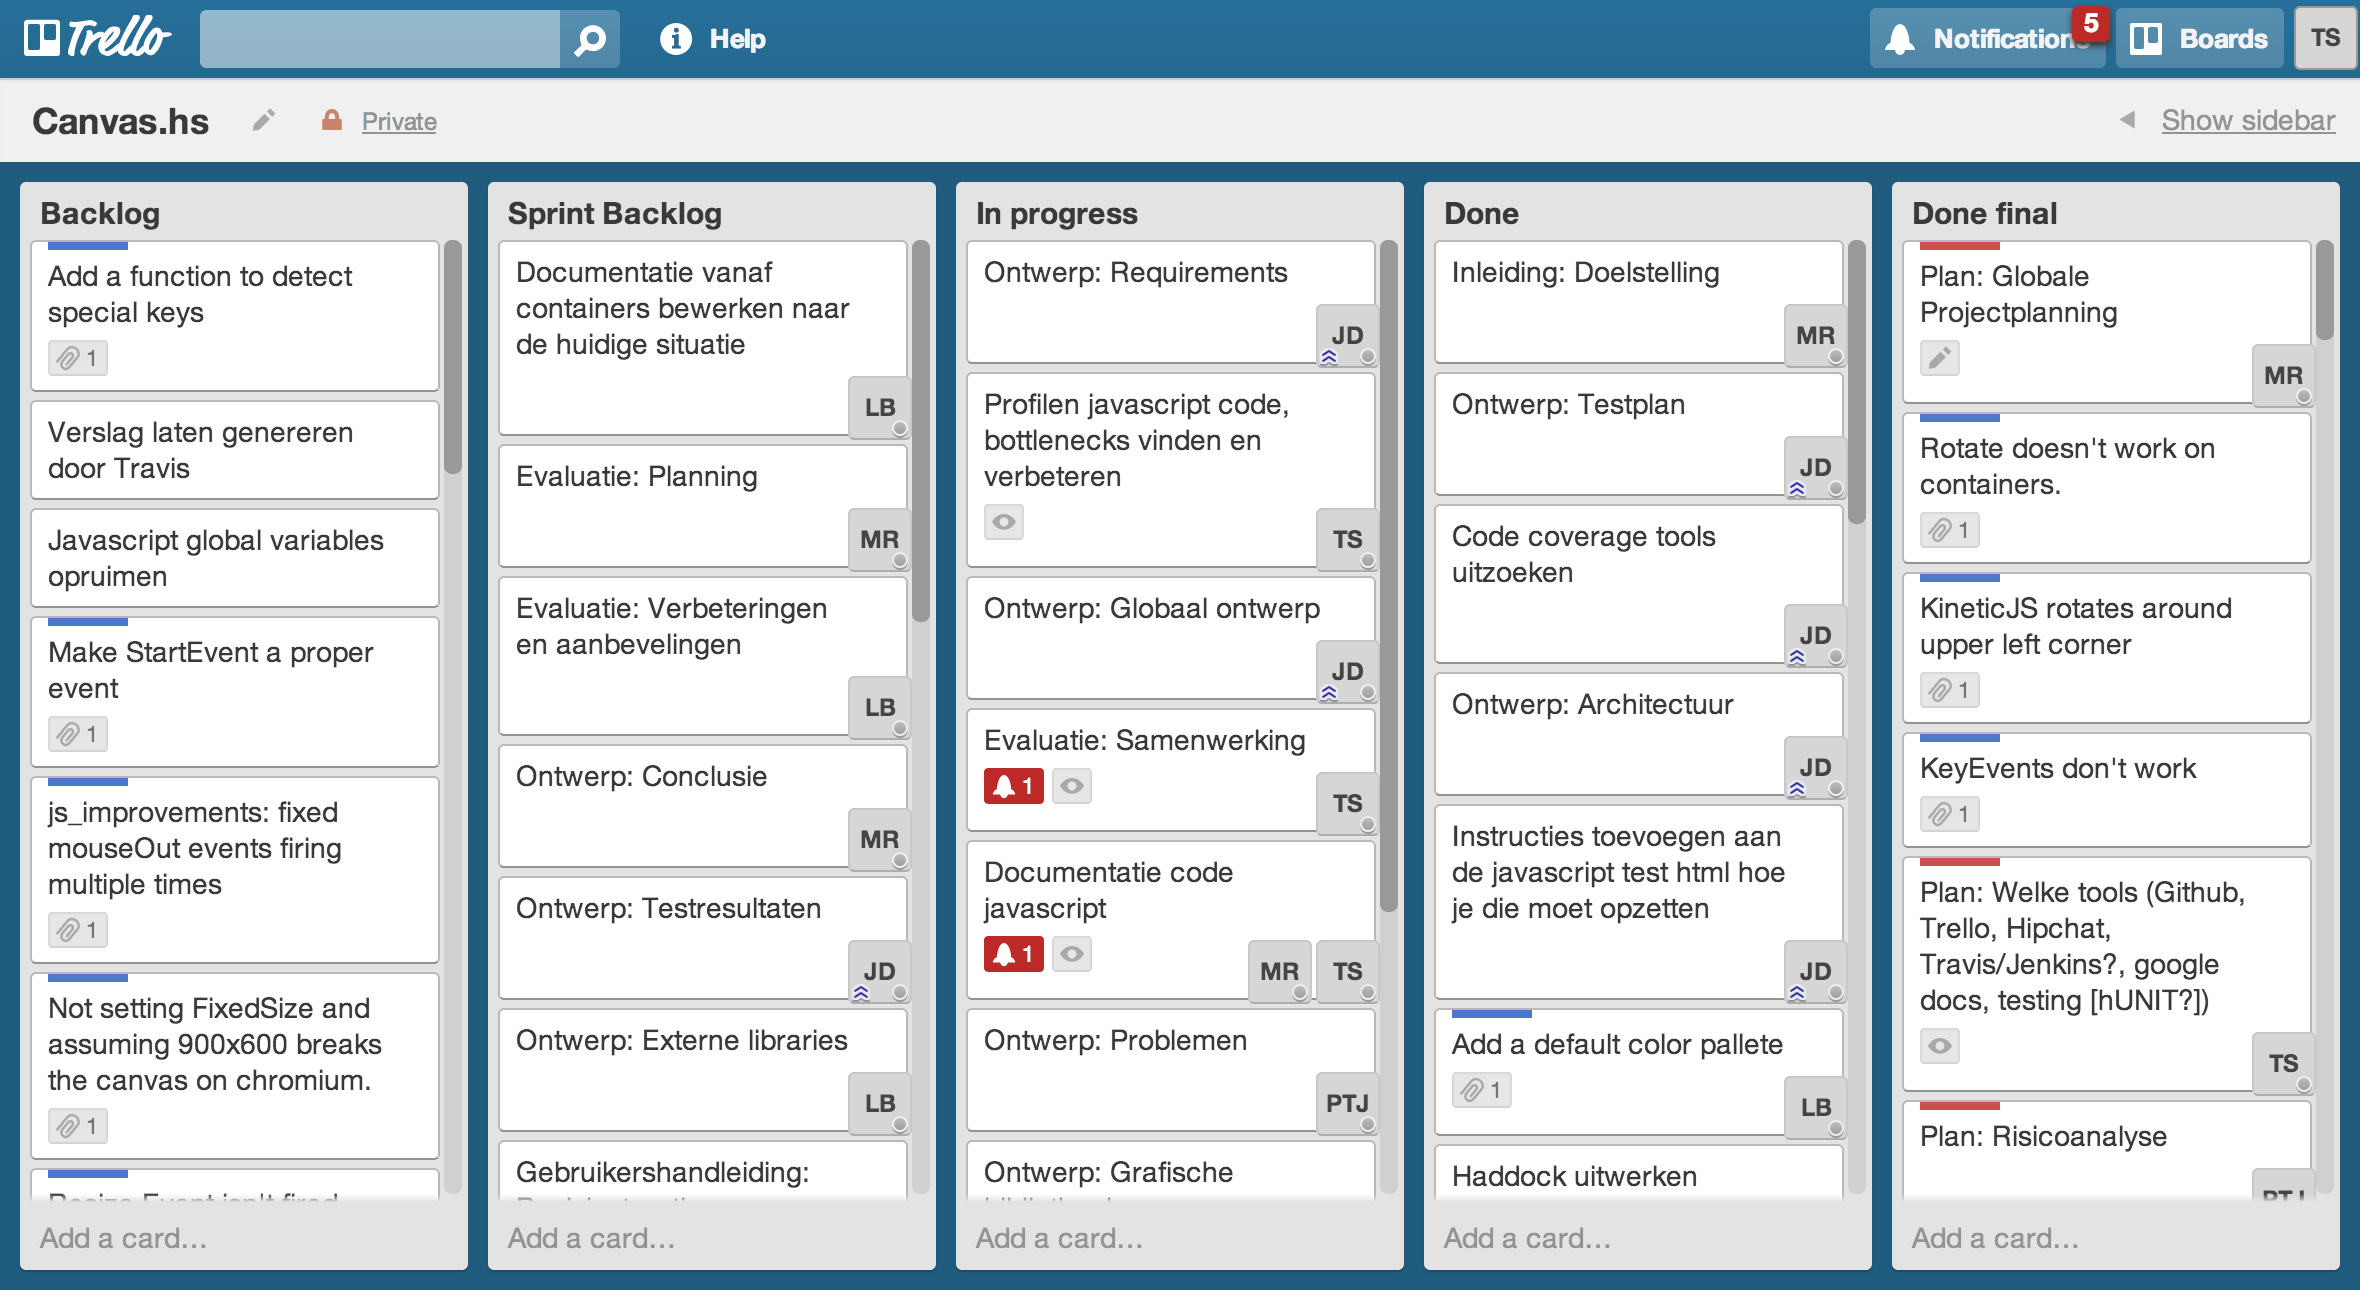
\includegraphics[keepaspectratio,width=\textwidth]{./images/trello.png}
\caption{Trello board}
\label{fig:trello}
\end{center}
\end{figure}

De lijst van ontwikkeltaken wordt bijgehouden op het \emph{GitHub} platform --{hier-over} meer in \fullref{sec:technische_organisatie}. Deze ontwikkeltaken worden op GitHub \emph{issues} genoemd. Ontwikkeltaken en andere taken worden gezamenlijk bijgehouden op \emph{Trello}. Met Trello kan een online takenbord gemaakt worden waarop de taken verdeeld zijn over de verschillende backlogs. In \autoref{fig:trello} is te zien welke status een taak heeft aan de kolom waar deze in staat. Mogelijke statussen van een taak zijn: in de Backlog, in de Sprint Backlog, In progress, Done of Done final. Hieronder wordt na het kopje \emph{Planning} besproken wat deze statussen inhouden. Door het gebruik van Trello hebben alle betrokkenen een goed inzicht in de taken die nog openstaan en de taken die reeds zijn uitgevoerd. Dit vergemakkelijkt vooral de taken van de scrummaster.

\subsubsection{Planning}
Bij scrum wordt gebruikt gemaakt van sprints. Dit zijn korte termijnen van --in ons geval-- twee weken waarbinnen een aantal features toegevoegd worden aan het bestaande systeem. Voorafgaand aan elke sprint wordt bepaald welke features in de komende sprint geïmplementeerd zullen worden. Als er tijdens een sprint nieuwe taken bedacht worden, dan worden deze op de backlog gezet voor volgende sprints.

Bij aanvang van een nieuwe fase wordt een planning gemaakt op basis van de taken in de project backlog. De prioriteit per taak wordt aangegeven door de \emph{product owner}, in ons geval de opdrachtgever. De teamleden bepalen vervolgens tijdens de sprintbespreking hoeveel van deze taken uitgevoerd kunnen worden in de komende sprint en verplaatsen deze naar het sprint backlog.

Bij elke samenkomst wordt een \emph{Scrum bespreking} gehouden. Tijdens deze bespreking vertelt ieder teamlid kort wat hij sinds de vorige bespreking gedaan heeft en of er problemen waren. Daarna vertelt het teamlid waar hij na de bespreking mee bezig gaat. Het is hier de bedoeling dat ieder teamlid een concreet korte termijn doel stelt. Door deze updates kan de scrum master bijhouden of de planning van de huidige sprint haalbaar is of dat er ingegrepen moet worden.

\section{Technische organisatie} \label{sec:technische_organisatie}
Bij het bouwen van software met een groep is het belangrijk dat elke ontwikkelaar zich kan concentreren op de feature die hij aan het ontwikkelen is. Idealiter hoeft er geen rekening gehouden te worden met andere features die door anderen ontwikkeld worden. Er is daarom gekozen om gebruik te maken van het gedistribueerde versiebeheer systeem \emph{Git} met een centrale repository op GitHub.

Er zijn afspraken gemaakt over hoe deze versiebeheer software gebuikt moet worden. Zo is er gebruik gemaakt van het \emph{branching model} Gitflow \cite{Gitflow2010}. Als een bepaalde versie van de software op een bepaalde branch staat, zegt dit iets over de status van die versie. Zo kan er begonnen worden aan een nieuwe feature vanaf de \inlinecode{dev} branch. Terwijl een versie die op de \inlinecode{master} branch klaar is voor gebruik. Het insturen van een nieuwe versie wordt een \emph{commit} genoemd.

Om voldoende code coverage te garanderen moet alle ontwikkelde code gecontroleerd zijn op het hebben van tests voordat het in de centrale development branch geplaatst mag worden. Dit gebeurt op de feature branches.  Iedere feature wordt in een aparte branch ontwikkeld en voordat een feature branch gemerged mag worden naar de dev branch, moet een pull request gemaakt worden op GitHub. Deze pull request wordt dan beoordeeld door twee andere personen op code coverage, code netheid en documentatie. Wanneer dit in orde is wordt de code gemerged naar de dev branch. Zie  \autoref{fig:branching} voor een overzicht van de branchingstrategie. Over de branchingstrategie wordt meer uitgelegd in de volgende sectie over pull requests.

\begin{figure}
\begin{center}
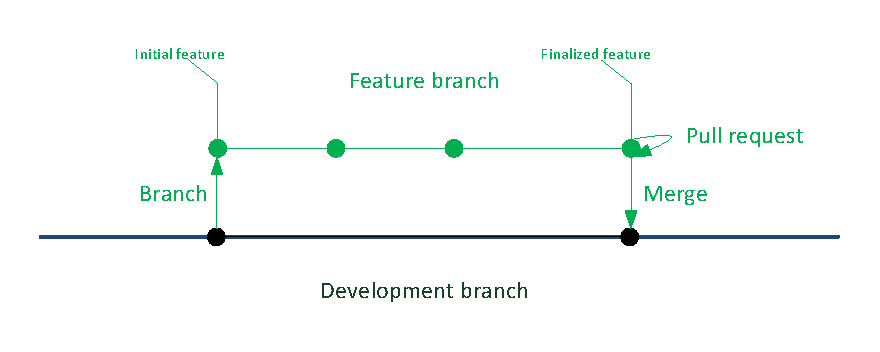
\includegraphics[keepaspectratio,width=\textwidth]{./images/branching.pdf}
\caption{Branching strategie van Canvas.hs}
\label{fig:branching}
\end{center}
\end{figure}

Door deze manier van werken is de development branch altijd goed getest en is het altijd mogelijk om een nieuwe release uit te brengen met de, op dat moment, volledig geteste features. Iedere release wordt in de master branch uitgebracht.

\subsubsection{Pull requests}
Bij aanvang van de ontwikkeling van een nieuwe feature wordt er een nieuwe branch gemaakt vanaf de \inlinecode{dev} branch. In \autoref{sec:shapesext} staat beschreven hoe \inlinecode{Arc} shapes toegevoegd kunnen worden. Dit is gebeurd op een aparte branch die begonnen is vanaf de \inlinecode{dev} branch. In dit geval zou die branch de \inlinecode{arcs} branch genoemd kunnen worden.

Als een feature af is moet deze beoordeeld worden door twee andere teamleden voordat de feature samengevoegd kan worden met de \inlinecode{dev} branch. Om dit te bewerkstelligen wordt gebruik gemaakt van een \emph{pull request} op GitHub zoals in \autoref{fig:pullrequest} getoond wordt. Deze pull request bevat informatie over de wijzigingen ten opzichte van de versie die op de \inlinecode{dev} branch staat. Een beoordelaar kan de code lezen en deze goedkeuren. Op het moment dat de code wordt goedgekeurd komt de nieuwe code met de toegevoegde feature op de \inlinecode{dev} branch te staan.

\begin{figure}
\begin{center}
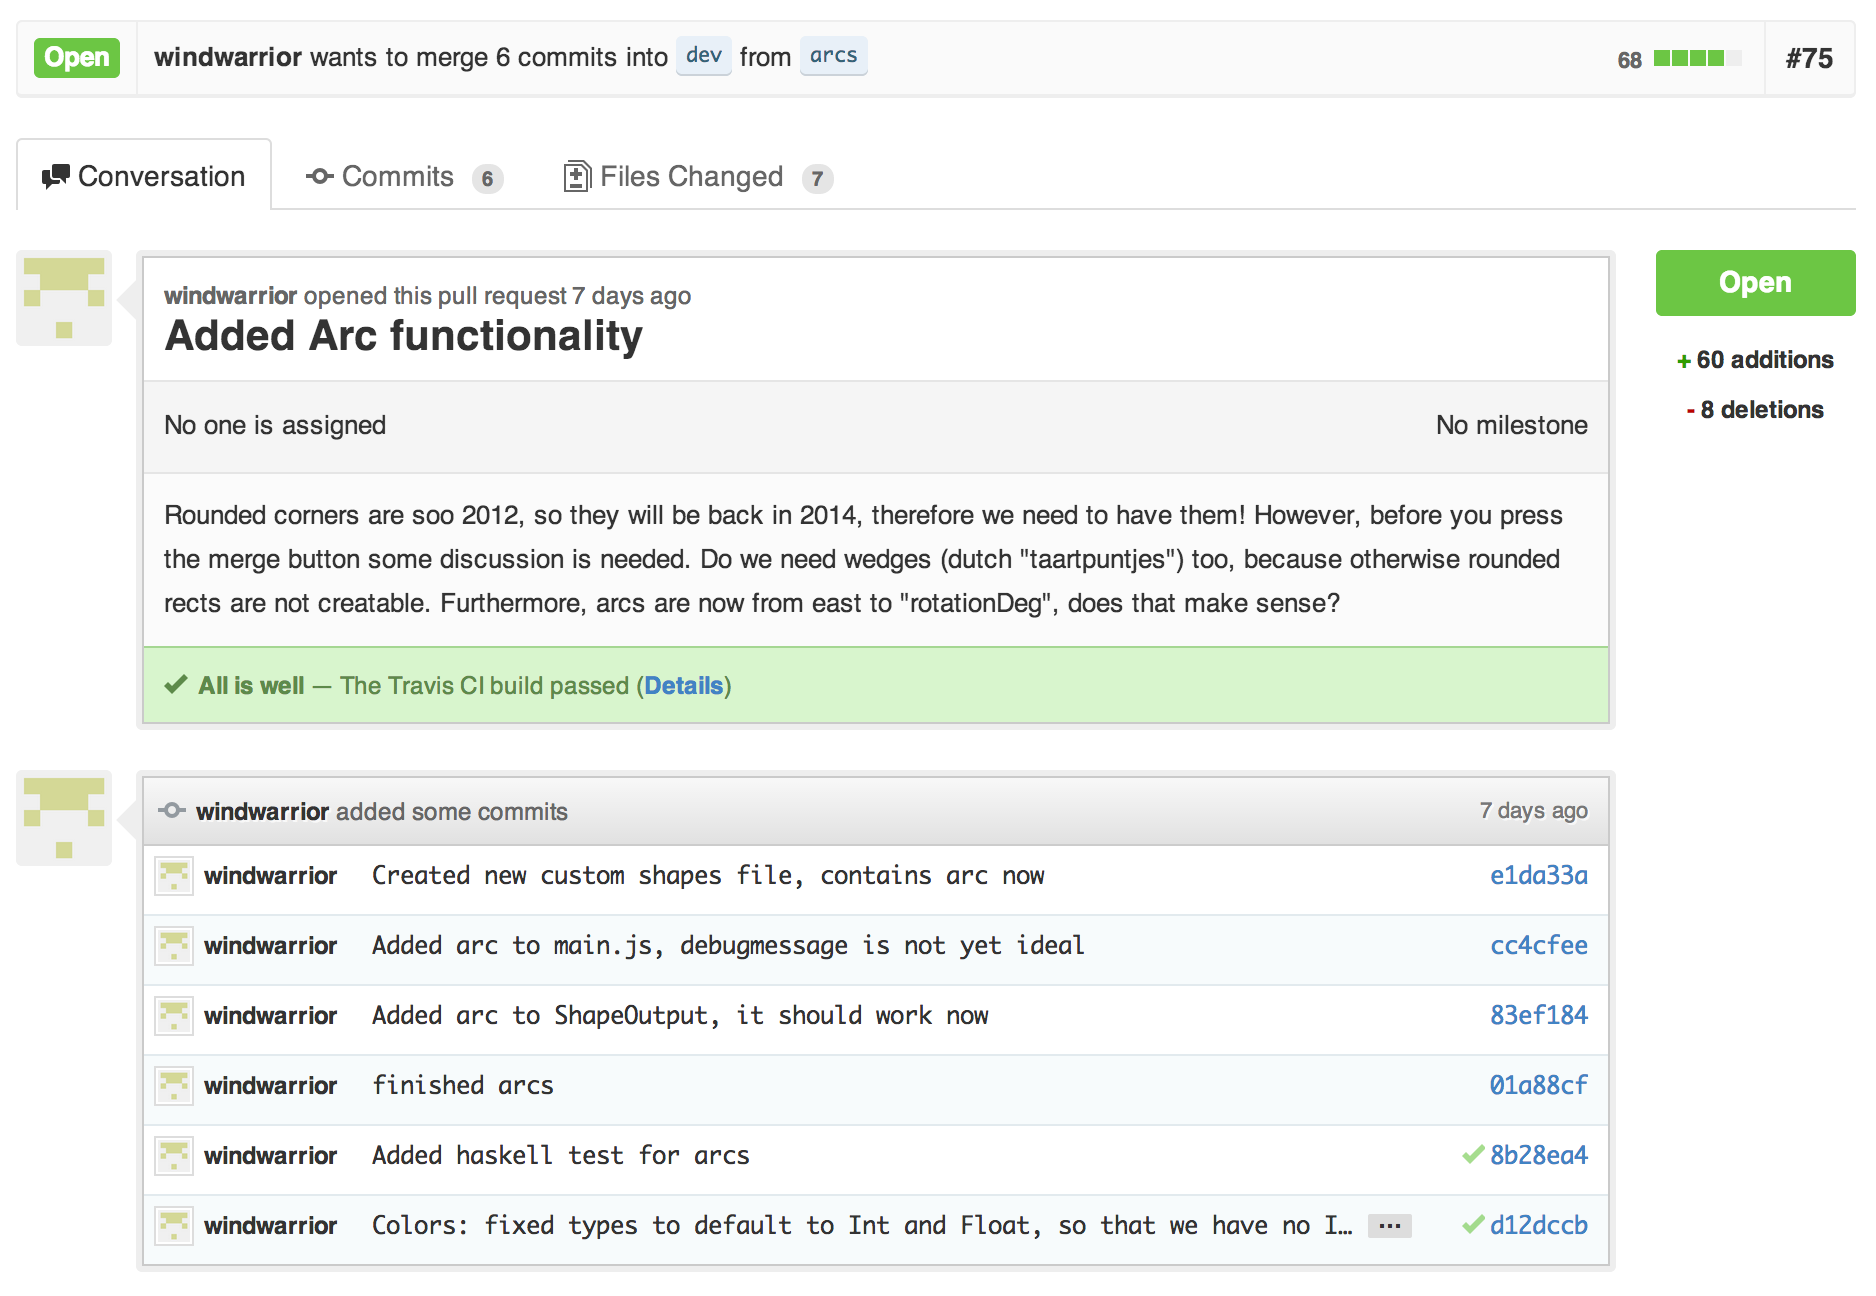
\includegraphics[keepaspectratio,width=\textwidth]{./images/pullrequest.png}
\caption{Pull Request \#75 Arcs geimplementeerd. – \url{https://github.com/CanvasHS/Canvas.hs/pull/75}}
\label{fig:pullrequest}
\end{center}
\end{figure}

\subsubsection{Continuous integration met Travis CI}
Om het beoordelen van code gemakkelijk te maken, is er gebruik gemaakt van de \emph{continuous integration} software \emph{Travis CI}. Deze software ziet of er nieuwe commits naar de centrale repository op GitHub gedaan zijn. Na het insturen van een nieuwe versie naar de centrale repository wordt er door Travis CI een virtuele machine opgestart. Deze machine downloadt de zojuist ingestuurde versie en compileert deze inclusief alle tests met een \emph{buildscript}. Dit buildscript staat in de root directory van de repository. Als het compileren slaagt en als alle tests slagen, dan zal de build als geslaagd worden gemarkeerd. In \autoref{fig:pullrequest} staat een groen vinkje op de laatste regel dat aangeeft dat de build slaagde na de laatste commit op de \inlinecode{arcs} branch. Mocht één van de tests niet slagen of het compileren niet slagen, dan wordt de build als mislukt gemarkeerd.

\begin{figure}[H]
\begin{center}
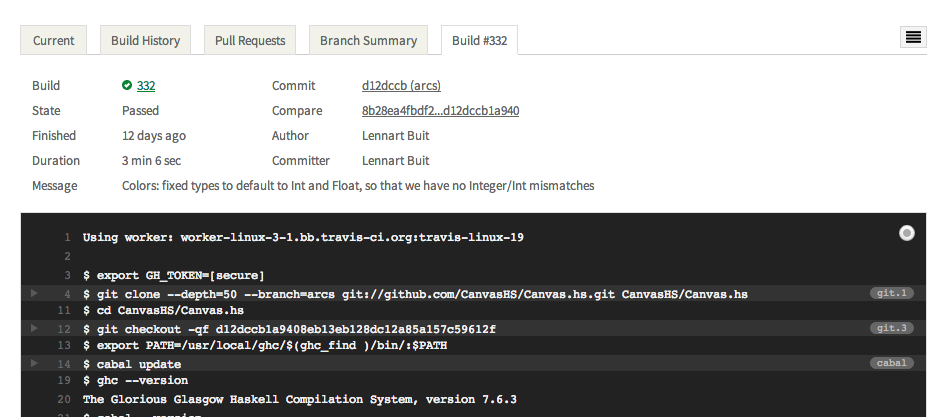
\includegraphics[keepaspectratio,width=\textwidth]{./images/travis.png}
\caption{Build van Pull Request \#75. – \url{https://travis-ci.org/CanvasHS/Canvas.hs/builds/16168834}}
\label{fig:travis}
\end{center}
\end{figure}

Informatie over het resultaat van een build kan gebruikt worden bij het beoordelen van een pull request. Als een beoordelaar ziet dat de build uit een pull request succesvol is, heeft hij een goede indicatie dat de pull request veilig gemerged kan worden.

Het buildscript voert naast de compilatie nog een paar functies uit. Zo genereert het buildscript ook de documentatie en uploadt het buildscript deze naar de Canvas.hs website, \url{http://canvashs.github.io}. Op de website kan de documentatie bekeken worden per build. Hierdoor hoeven ontwikkelaars zelf geen documentatie meer te genereren en hebben zij altijd de laatste documentatie.

\section{Conclusie}
Met duidelijke afspraken over project- en technische organisatie is er een basis voor het ontwerpen en ontwikkelen van Canvas.hs. \autoref{hoofdstuk:evaluatie} beschrijft de evaluatie en reflecteert op het toepassen van de in dit hoofdstuk beschreven organisatievormen en -technieken. 
